\documentclass[11pt,letterpaper]{article}
\input{G:/Dropbox/Math/preamble}
\usepackage{fullpage}
\usepackage{multicol}

\begin{document}
\flushleft
\begin{multicols}{2}

\begin{large}\textbf{Math 2554 Quiz 3: $\oint $ 2.6-2.7 \\
Tues 16 Sep 2014}\end{large}

\hfill\textbf{Name:  }\underline{\hspace{17ex} KEY\hspace{17ex}}

\vspace{.5in}

\end{multicols}

\pagestyle{empty}

\flushleft

You have 20 minutes to complete this quiz.  Eyes on your own paper and good luck!

\begin{enumerate}
\item  \textbf{Definitions/Concepts.} 
\begin{enumerate}
\item (3 pts) The function $f$ is {\bf continuous at the point $a$} means it satisfies the Continuity Checklist:

\vspace{1pc}
%\vspace{6pc}
SOLUTION:
\begin{enumerate}[1.]
\item $f(a)$ is defined ($a$ is in the domain of $f$).
\item $\lim_{x\to a}f(x)$ exists.
\item $\lim_{x\to a}f(x)=f(a)$ (the value of $f$ equals the limit of $f$ at $a$).
\end{enumerate}

\vspace{1pc}
\item (2 pts) ``The limit of $f(x)$ as $x$ approaches $a$ equals $L$" means that for any positive number $\epsilon$, there is another positive number $\delta$ such that

\vspace{1pc}
SOLUTION: \hspace{5ex}$|f(x)-L|<\epsilon\qquad\text{whenever}\qquad 0<|x-a|<\delta$.
%\begin{center}\underline{\hspace{15ex}}\hspace{5ex}whenever\hspace{5ex}\underline{\hspace{15ex}}\end{center}
\end{enumerate}

\vspace{1pc}
\item \textbf{Questions/Problems.} Suppose $\lim_{x\to 3}f(x)=4$, where $f$ is the function in Figure 1.

\vspace{-1pc}  
\begin{figure}[h]
\begin{center}
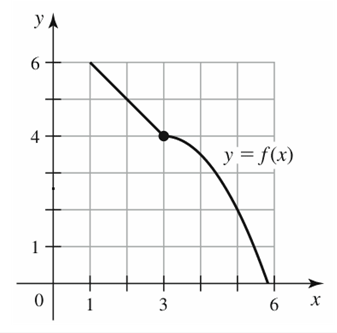
\includegraphics[scale=0.6]{Q3pic.png}
\caption{$f(x)$ (Briggs, W. and Cochran, L. \emph{Calculus: Early Transcendentals}, p. 116)}
\end{center}
\end{figure}

\vspace{-0.5pc}
What must $\delta$ equal in order to satisfy $|f(x)-4|<\epsilon$ whenever $0<|x-3|<\delta$, for 
\begin{enumerate}
\item (1 pt) $\epsilon=2$?

\vspace{0.5pc}
SOLUTION: 2

\vspace{0.5pc}
\item (1 pt) $\epsilon=\frac{1}{2}$?

\vspace{0.5pc}
SOLUTION: $\frac{1}{2}$

\hfill {\bf\Large MORE ON THE NEXT PAGE $\to$}

\vspace{0.5pc}
\item (1 pt) Write a formula for $\delta$ in terms of $\epsilon$ that works, once $\epsilon$ gets small enough.

\vspace{0.5pc}
SOLUTION: $\delta=\epsilon$

\vspace{0.5pc}
\item (ChAlLeNgE pRoBlEm) Justify your answer to (c).

\vspace{0.5pc}
SOLUTION: To the left of $x=3$, $f(x)$ is linear, so $\delta\sim\epsilon$.  To the right of $x=3$, $f(x)$ is quadratic, so $\delta\sim\sqrt\epsilon$.  Once $\epsilon$ gets smaller than 1, $\sqrt\epsilon>\epsilon$.  This means the smaller value for $\delta$ will be on the linear side of $x=3$.
\end{enumerate}

\vspace{1pc}
\item \textbf{Computations/Algebra.} (2 pts) Let 
\[g(x)=\begin{cases}\frac{x^2+3x+2}{x+1} & x\neq -1 \\
	k & x=-1 
    \end{cases}.\]
Using the Continuity Checklist, find the value of $k$ that makes $g$ continuous at the point $-1$.  

\vspace{1pc}
SOLUTION: In the Continuity Checklist, $g(-1)$ is defined (as $k$).  We compute,
\begin{align*}\lim_{x\to -1}g(x) &= \lim_{x\to -1}\frac{x^2+3x+2}{x+1} \\
 &= \lim_{x\to -1}\frac{(x+2)(x+1)}{x+1} \\
 &= \lim_{x\to -1}x+2 \\
 &= (-1)+2 =1\quad\text{ exists;}
\end{align*}
and finally we set
\[g(-1)=k=\lim_{x\to -1}g(x)=1.\]

\end{enumerate}

\end{document}


